%%UTF-8
\documentclass{standalone}
    \usepackage{tikz}
    \usetikzlibrary{matrix,chains,positioning,decorations.pathreplacing,arrows}
    \begin{document}
    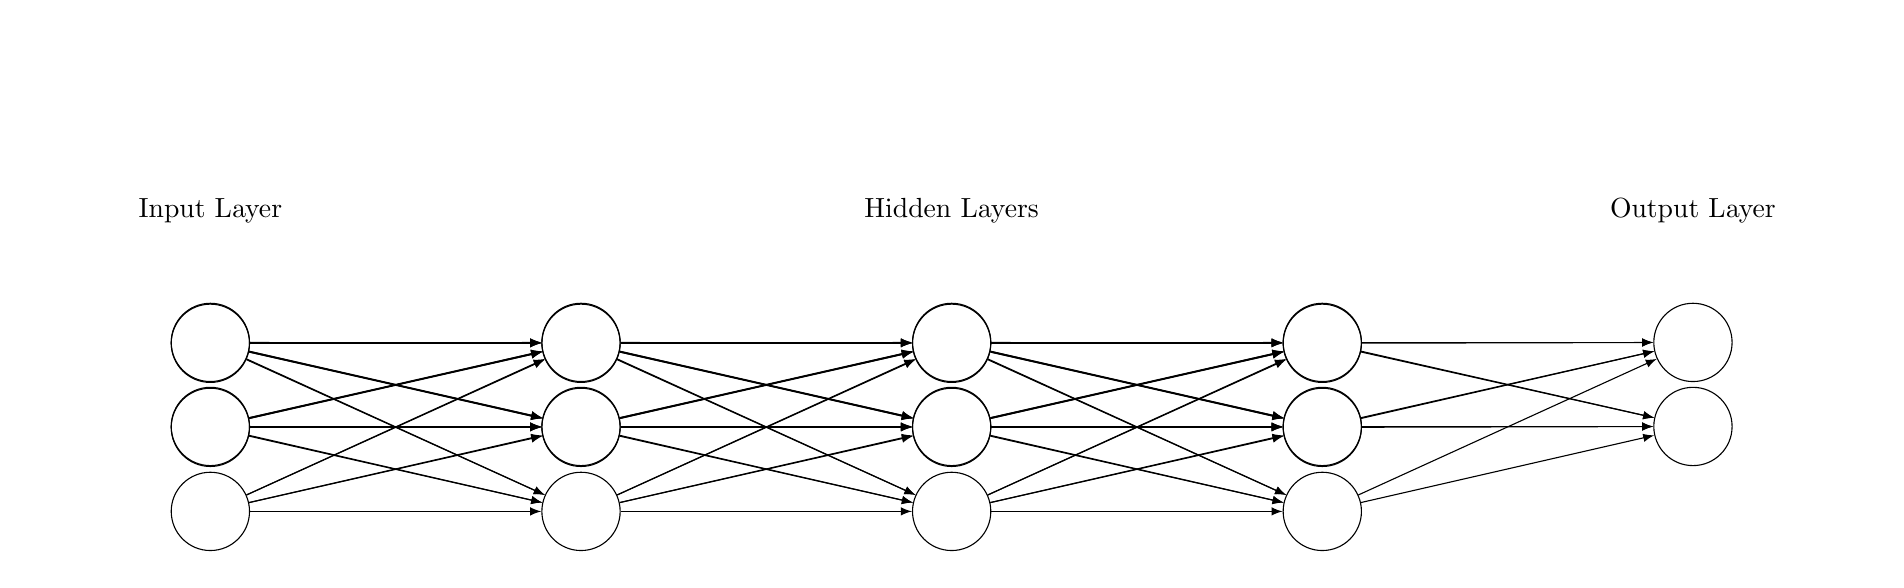
\begin{tikzpicture}[
        plain/.style={
          draw=none,
          fill=none,
          row sep=-29pt          
          },
        net/.style={
          matrix of nodes,
          nodes={
            draw,
            circle,
            inner sep=10pt
            },
          nodes in empty cells,
          column sep=2cm,
          row sep=2pt
          },
        >=latex
        ]
        \matrix[net] (mat)
        {
        |[plain]| \parbox{3.6cm}{\centering Input Layer} &|[plain]| & |[plain]| \parbox{3.6cm}{\centering Hidden Layers} &|[plain]| & |[plain]| \parbox{3.6cm}{\centering Output Layer} \\
        & & & & |[plain]| \\
        & & & & \\
        & & & & |[plain]| \\
        & & & & \\
        & & & & |[plain]| \\
        };
        % \foreach \ai [count=\mi ]in {2,4,6}
            % node at (mat-\ai-1) {$x_\mi$};
        %   \draw[<-] (mat-\ai-1) -- node {Input \mi} +(-2cm,0);
        \foreach \ai in {2,3,...,6}
        {\foreach \aii in {2,3,...,6}
          \draw[->] (mat-\ai-1) -- (mat-\aii-2);
        }
        \foreach \ai in {2,3,...,6}
        {\foreach \aii in {2,3,...,6}
          \draw[->] (mat-\ai-2) -- (mat-\aii-3);
        }
        \foreach \ai in {2,3,...,6}
        {\foreach \aii in {2,3,...,6}
          \draw[->] (mat-\ai-3) -- (mat-\aii-4);
        }
        \foreach \ai in {2,3,...,6}
        {\foreach \aii in {3,5}
          \draw[->] (mat-\ai-4) -- (mat-\aii-5);
        }
        % \foreach \ai [count=\mi] in {2,4,...,6}
        %   \draw[->] (mat-\ai-2) -- node[near start] {$a_\mi^{(2)}$} (mat-5-3);
        %   \draw[->] (mat-8-2) -- (mat-5-3);
        %   \draw[->] (mat-5-3) -- node[above] {$h_{w,b}(x)$} +(2cm,0);
        \end{tikzpicture}
    \end{document}